\documentclass[11pt]{article}
\usepackage[a4paper,margin=25mm]{geometry}
\usepackage{graphicx,amsmath,amssymb,amsthm,booktabs,multirow,float}
\usepackage[T1]{fontenc}\usepackage{lmodern,microtype}
\usepackage[round,authoryear]{natbib}\setcitestyle{aysep={}}\usepackage{hyperref,xurl}
\providecommand{\doi}[1]{\url{https://doi.org/#1}}
\input{glyphtounicode}\pdfgentounicode=1
\theoremstyle{plain}
\newtheorem{theorem}{Theorem}\newtheorem{proposition}[theorem]{Proposition}\newtheorem{lemma}[theorem]{Lemma}
\theoremstyle{definition}\newtheorem{remark}{Remark}\newtheorem{example}{Example}
\newcommand{\T}{\mathcal T}\newcommand{\Pp}{\mathbb P}\newcommand{\E}{\mathbb E}\newcommand{\ind}{\mathbf1}
\newif\ifanonymous\ifdefined\blindversion\anonymoustrue\else\anonymousfalse\fi
\newsavebox{\resultsbox}
\raggedbottom\setlength{\emergencystretch}{2em}
\hypersetup{colorlinks=true,linkcolor=black,citecolor=black,urlcolor=blue,pdftitle={Certified degree bounds and shared hubs in correlation spanning trees}}
\title{Certified degree bounds and shared hubs in correlation spanning trees}
\ifanonymous
\author{}\hypersetup{pdfauthor={}}
\else
\author{Marek Ga\l{}\k{a}zka\textsuperscript{1}\thanks{Corresponding author: galazka@amu.edu.pl}\quad Hanna Wdowicka\textsuperscript{2}\\[5pt]
\small\textsuperscript{1}Faculty of Mathematics and Computer Science,\\[-2pt]
\small Adam Mickiewicz University, Pozna\'n, Poland\\[3pt]
\small\textsuperscript{2}Department of Statistics, Pozna\'n University of Economics and Business, Poland}
\hypersetup{pdfauthor={Marek Galazka and Hanna Wdowicka}}
\fi
\date{}
\begin{document}
\maketitle
\begin{abstract}
Which variables are demonstrably most connected, and when must they share that status? We construct simultaneous degree bounds and hub statements for population correlation spanning trees. An independent training sample selects a reference tree, useful Kendall tau-a comparisons, their testing sequence and betting fractions. Verification on the remaining observations retains finite-sample familywise error control under independent and identically distributed sampling, including ties. Classical tree constraints project the certified comparisons into degrees; exact enumeration audits the remaining relaxation loss. In a fresh validation study of 6600 simulated datasets, the selected procedure identifies the unique hub in 70.3\% of Gaussian and 40.0\% of heavy-tailed separated-star samples (300 datasets each, 12 vertices, 1008 observations), compared with zero for fixed-family matching evidence. The asymptotic multiplier comparator is more powerful in these cells. In 35079 complete adult responses to a ten-item self-esteem questionnaire, the selected procedure determines eight degrees exactly and certifies three shared hub members. Fixed-family evidence leaves a unique hub possible. Independent enumeration verifies the two retained trees. The shared-hub conclusion recurs in 16 of 100 additional random splits, revealing substantial split sensitivity. The improvement is conditional on informative selection: short samples and near-tied leaders remain difficult. This separates useful structural decisions from numerical interval tightening and distinguishes shared hub status from an unresolved unique-hub claim.
\end{abstract}
\noindent\textbf{Keywords:} Kendall tau-a; e-values; sample splitting; simultaneous inference; multiple testing; ordinal data.

\section{Introduction}
When a network summarizes relationships among measurements, can its most connected variable really be singled out? A spanning tree connects all variables with no cycles. A variable's degree counts its links, and a hub has the largest degree. Estimated correlations can make a variable look central even when the data do not distinguish it from its competitors. Conversely, an interval containing several ranks can reflect a well-established tie between hub degrees rather than an absence of information.

We develop and evaluate a procedure that selects a manageable set of useful edge comparisons on independent training observations, verifies them on held-out observations, and converts them into simultaneous statements about degrees and hubs. Training fixes the reference tree, comparison order and betting fractions. A fixed sequence stops at its first failed verification, preserving familywise error control without testing every comparison at a large-family Bonferroni threshold. The statistical ingredients are established betting and multiple-testing principles; the contribution is their explicit tree-directed construction, its conditional validity and power analysis, and a matched demonstration of changed structural conclusions.

The questionnaire example illustrates the distinction. With ten ordinal items, fixed-family evidence permits three trees, including one with a unique hub. Independently selected inference retains two trees and determines eight degrees exactly. In both trees, Q1, Q3 and Q10 have degree three, and no item has a larger degree. Thus the procedure certifies shared maximum-degree membership and excludes a unique hub (Figure~\ref{fig:intro}). The degree result follows already from the screened tree family; expensive pair optimization is unnecessary in this example. This displayed split is favourable: the three-member conclusion recurs in only 16 of 100 additional random splits.

\begin{figure}[htbp]\centering
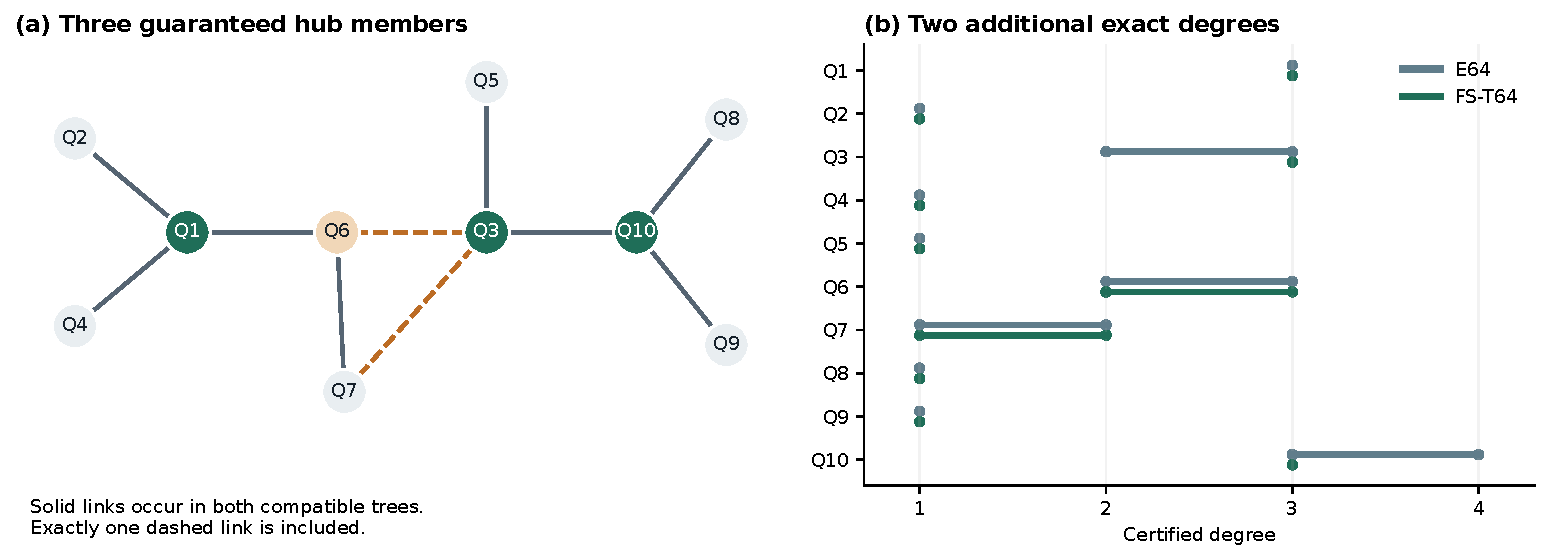
\includegraphics[width=\textwidth]{Fig1.pdf}
\caption{A structural conclusion in 35079 complete adult questionnaire responses. Green nodes are guaranteed members of the maximum-degree set under FS-T64. Exactly one dashed link completes each of the two compatible trees. The degree bounds for Q3 and Q10 become exact compared with E64. These are within-procedure nominal 95\% statements for the signed tau-a tree under the IID working model. The displayed split is favourable: all three memberships recur together in 16 of 100 additional splits. They do not identify psychological causes or clinical targets.}\label{fig:intro}
\end{figure}

The power comparison uses fresh data rather than the pilot used to select the procedure. At 1008 observations, unique-hub certification rises from zero with E64 to 70.3\% in the separated Gaussian star and 40.0\% under heavy tails. The full-U-statistic multiplier comparator remains more powerful, reaching 100\% in both cells. The finite-sample construction therefore addresses a different accuracy requirement; it does not dominate every alternative. At 252 observations and in near-tied leader models, the selected procedure still fails to identify a unique hub.

The optimization foundations are classical. Interval robust spanning trees, possible or necessary optimality, and robust dependence trees are studied by \citet{yaman2001,kasperski2007,fortin2007,zaffalon2005}; sensitivity analysis supplies further algorithmic context \citep{pettie2015}. Our input is a calibrated relation between population edges, rather than independent intervals supplied to an optimization problem. Cut/cycle screening, matroid rank identities and weak duality convert that relation into vertex information. Exact small-graph audits quantify what these relaxations lose. Rank inference must preserve ties \citep{hall2009,mogstad2024}, while combinatorial inference under graphical-model assumptions addresses related but different targets \citep{neykov2019}.

Correlation trees originate in applications including financial networks \citep{mantegna1999,galazka2011}. Bootstrap edge reliability and centrality stability provide valuable descriptive references \citep{tumminello2007,musciotto2018,epskamp2018}. Here a degree certificate concerns every population-optimal tree on a simultaneous coverage event. It differs from an edge's resampling frequency, and from centrality in a partial-correlation network. Online Resource 1 contains the full morphometric comparison, financial sensitivity study and bootstrap diagnostics.
\section{Population target and simultaneous orders}
Let $G=(V,E)$ be a fixed connected graph with $p\ge2$ vertices and $m$ edges. For weights $w$, let
\[
 \T(w)=\arg\max_{T\text{ spanning tree}}\sum_{e\in T}w_e.
\]
In the correlation application $G$ is complete. A maximum-correlation tree has the same optimal-tree family as the minimum-distance tree based on $\sqrt{2(1-w_e)}$: both are determined by the same edge ordering, including ties. Strictly increasing edge transformations preserve this family.

\paragraph{Relation to dependence trees.}
Chow--Liu trees maximize pairwise mutual information when approximating a distribution by a tree factorization \citep{chow1968}. For Gaussian variables, mutual information is $-\tfrac12\log(1-\rho^2)$ and therefore orders edges by $|\rho|$, whereas our target orders signed correlations. For continuous Gaussian-copula models, $\tau=2\arcsin(\rho)/\pi$ connects Kendall weights with latent correlations \citep{liu2012}. Under a correctly specified faithful Gaussian tree model, the corresponding absolute-correlation tree recovers graphical neighbours and degrees count those neighbours. These additional assumptions are not imposed on the ordinal questionnaire. Its signed marginal-association tree is a descriptive population target, and changes in coding or tie normalization can change that target.

\paragraph{Pearson and Kendall targets.}
Gaussian and $t_5$ correlations have the same edge ordering as their Kendall weights, but this relation need not extend to a nonelliptical population. For a concrete construction, start with the $p=12$ separated Gaussian star below and set $Y_i=\exp(\sigma_i X_i)$, where $\sigma_0=2.5$ and the other scales span $[0.3,1.5]$. Monotonicity leaves every Kendall kernel unchanged. The normal exponential moment formula gives
\[
 \rho^{Y}_{ij}=\frac{\exp(\sigma_i\sigma_j\rho^X_{ij})-1}{\sqrt{(\exp(\sigma_i^2)-1)(\exp(\sigma_j^2)-1)}}.
\]
The Kendall tree has vertex-zero degree 11, whereas the Pearson tree has vertex-zero degree 1. The supplied verifier checks both population trees and kernel invariance. Thus the weight definition is part of the inferential target.

Write $S_i=\{e:i\in e\}$ and $d_i(T)=|T\cap S_i|$. Descending ranks of vertex $i$, including every resolution of equal degrees, range from
\begin{equation}\label{eq:ranks}
 r_i^-(T)=1+\sum_{j\ne i}\ind\{d_j(T)>d_i(T)\},\qquad
 r_i^+(T)=p-\sum_{j\ne i}\ind\{d_j(T)<d_i(T)\}.
\end{equation}
A hub member belongs to $H(T)=\{i:d_i(T)=\max_jd_j(T)\}$; it need not be unique. For a retained family $\mathcal F$, $\bigcap_{T\in\mathcal F}H(T)$ contains the guaranteed hub members. The sufficient condition $\underline d_i\ge\max_{j\ne i}\overline d_j$ also certifies membership. Two guaranteed members exclude a unique hub even when each tied-rank interval includes several positions.

The inferential target contains these quantities for every $T\in\T(w_0)$. Under complete independence all edges have weight zero, every labelled tree is optimal, and the appropriate degree and rank targets are $[1,p-1]$ and $[1,p]$. Selecting one arbitrary tied optimum would artificially narrow this target.

A random strict relation $\widehat{\succ}$ is simultaneously valid if
\begin{equation}\label{eq:event}
 \Pp(\mathcal E)\ge1-\alpha,\qquad
 \mathcal E=\{e\widehat{\succ}f\Longrightarrow w_{0e}>w_{0f}\text{ for all }e,f\}.
\end{equation}
We may take its transitive closure without an additional error budget. Every computational restriction below is conditional on this same event. The relation need not specify all pairwise edge comparisons, and its incompleteness is a source of conservative bounds.

\section{An exact Kendall comparison construction}\label{sec:kendall}
Suppose $X_1,\ldots,X_n$ are IID $p$-vectors. Coordinates may be dependent or discrete, and no moment assumption is imposed. For independent copies $X,X'$, define
\[
 \tau_{ij}=\E[\operatorname{sgn}(X_i-X_i')\operatorname{sgn}(X_j-X_j')].
\]
This is Kendall tau-a, not the tie-normalized tau-b. Attach independent uniform random variables $U_{ti}$ to each observation and coordinate, and order $\widetilde X_{ti}=(X_{ti},U_{ti})$ lexicographically. Randomization is independent of the observed sample.

For a predetermined pairing $(1,2),(3,4),\ldots$, let $N=\lfloor n/2\rfloor$ and
\[
 S_{ki}=\operatorname{sgn}(\widetilde X_{2k-1,i}-\widetilde X_{2k,i}),\qquad
 H_{k,e}=S_{ki}S_{kj},\quad e=\{i,j\}.
\]
Here $H_{k,e}\in\{-1,1\}$ and the vectors $H_k$ are IID. For an ordered comparison $(e,f)$ set
\[
 \begin{aligned} A_{ef}&=\sum_k\ind\{H_{k,e}=1,H_{k,f}=-1\},\\
 B_{ef}&=\sum_k\ind\{H_{k,e}=-1,H_{k,f}=1\},\qquad D_{ef}=A_{ef}+B_{ef}.\end{aligned}
\]
The one-sided exact p-value is
\begin{equation}\label{eq:pvalue}
 p_{ef}=\Pp\{\operatorname{Bin}(D_{ef},1/2)\ge A_{ef}\},
\end{equation}
with value one when $D_{ef}=0$. This is the conditional McNemar test \citep{mcnemar1947}, applied to paired edge kernels.

For a fixed family of unordered edge pairs $\mathcal C$, we test both directions, giving $K=2|\mathcal C|$ hypotheses. The local family consists of distinct edges sharing a vertex and has $K=p(p-1)(p-2)$ on a complete graph. The complete family and its multiplicity cost are examined below. Apply Holm's step-down rule \citep{holm1979} at level $\alpha$: ordered p-values $p_{(k)}$ are rejected until the first failure of $p_{(k)}\le\alpha/(K-k+1)$. Rejections define $e\widehat{\succ}f$; subsequently take the transitive closure.

\begin{theorem}[Finite-sample order and hub coverage]\label{thm:finite}
For IID rows and the predetermined pairing above, the resulting relation satisfies \eqref{eq:event} with $w_{0e}=\tau_e$, for every finite $n\ge2$. The probability includes auxiliary tie randomization. Consequently, every degree, degree-difference and rank bound obtained by the valid outer projections in Sections~\ref{sec:minor}--\ref{sec:rank} covers its target simultaneously with probability at least $1-\alpha$, for all population-optimal trees and every resolution of degree ties.
\end{theorem}
\begin{proof}
Conditional on $X,X'$, if neither coordinate is tied, the augmented sign product equals the original sign product. If either is tied, the independent auxiliary sign for that coordinate has mean zero. Thus $\E H_{k,e}=\tau_e$, including when both coordinates tie. Put $\pi_+=\Pp(H_e=1,H_f=-1)$ and $\pi_-=\Pp(H_e=-1,H_f=1)$. Then $\tau_e-\tau_f=2(\pi_+-\pi_-)$. Conditional on $D_{ef}$, $A_{ef}$ is binomial with success probability $q=\pi_+/(\pi_++\pi_-)$ whenever the denominator is positive. Under $\tau_e\le\tau_f$, $q\le1/2$, so \eqref{eq:pvalue} is superuniform by binomial stochastic monotonicity. The zero-denominator case gives $D_{ef}=0$ almost surely. Holm's argument therefore controls the probability of any false strict order by $\alpha$, regardless of dependence among comparisons. Transitive consequences remain true on the same event. Each subsequent outer projection retains all population-optimal trees on that event, proving the final assertion.
\end{proof}

The pairing cannot be selected after inspecting which arrangement gives favorable tests. A fixed pairing, or independent random pairing, is valid; trying several and retaining the best requires additional multiplicity control. This construction deliberately uses $N$ independent pairs. The full-sample Kendall estimator uses all $n(n-1)/2$ pairs, whose kernels are dependent. Treating those kernels as independent would invalidate the binomial calculation. Applying the IID result to serially dependent financial returns or fitted residuals is also unjustified.

\begin{proposition}[A sufficient discordance-dependent power bound]\label{prop:power}
Consider $s\ge1$ selected true comparisons from the tested family. Suppose each has gap $\Delta=\tau_e-\tau_f\ge\delta>0$ and discordance probability $d=\Pp(H_e\ne H_f)\le\bar d$. If
\begin{equation}\label{eq:power}
 N\ge\frac{64\bar d}{\delta^2}\max\left\{\log\frac K\alpha,\log\frac{2s}\eta\right\},\qquad 0<\eta<1,
\end{equation}
then all these comparisons are rejected with probability at least $1-\eta$.
\end{proposition}
\begin{proof}
Let $Z_k=(H_{k,e}-H_{k,f})/2$. Its mean is $\Delta/2$, variance is at most $\bar d$, and its centered absolute value is at most two. Bernstein's inequality gives
\[
 \Pp\{A-B<N\delta/4\}
 \le \exp\{-N\delta^2/(32\bar d+16\delta/3)\}
 \le \exp\{-N\delta^2/(64\bar d)\},
\]
where $\delta\le2\bar d$. A second Bernstein bound gives $\Pp(D>2N\bar d)\le\exp(-3N\bar d/8)$. Outside these events, the binomial Hoeffding bound implies
\[
 p_{ef}\le\exp\{-(A-B)^2/(2D)\}\le\exp\{-N\delta^2/(64\bar d)\}.
\]
Put $t=N\delta^2/(64\bar d)$. Since $\delta^2\le4\bar d^2$, both bad-event probabilities are at most $e^{-t}$. Condition \eqref{eq:power} gives $e^{-t}\le\alpha/K$ and $2s e^{-t}\le\eta$. A union bound over the $s$ comparisons therefore gives the required probability, and every p-value at most $\alpha/K$ is rejected by Holm.
\end{proof}

The bound exhibits the role of discordance in simultaneous power. It is a sufficient condition; estimator efficiency and realized power are examined next.

\subsection{Exact evidence aggregation with deterministic tie handling}\label{sec:evalues}
P-value averaging can be conservative at a large comparison family. We therefore also aggregate nonnegative evidence with null expectation at most one, an e-value \citep{vovk2021}. For matching $r$, use the original tau-a kernels $K_{r,k,e}\in\{-1,0,1\}$, retaining zero at a tied coordinate, and set $Z_{r,k,ef}=(K_{r,k,e}-K_{r,k,f})/2\in[-1,1]$. For a predetermined fraction $0\le\lambda<1$, define
\[
 E_{r,\lambda,ef}=\prod_{k=1}^N(1+\lambda Z_{r,k,ef}).
\]
The evaluated multiset of seven fractions is
\[
 \Lambda_N=\{1/32,1/16,1/8,1/4,1/2,3/4,\min(1/2,N^{-1/2})\}.
\]
Its last element is determined by sample size and ensures consistency even for gaps too small for the fixed fractions. We compare $R=8$ and $R=64$ matchings, with the former nested in the latter, and put
\begin{equation}\label{eq:evalue}
 \overline E_{ef}=\frac1{7R}\sum_{r=1}^R\sum_{\lambda\in\Lambda_N}E_{r,\lambda,ef},\qquad
 p^E_{ef}=\min\{1,1/\overline E_{ef}\}.
\end{equation}
The averaging rule is classical e-value merging. Its use here combines exact Kendall contrast evidence across shared-observation matchings. The statistic handles ties directly, without auxiliary sign randomization.

\begin{proposition}[Finite-sample evidence validity and fixed-family consistency]\label{prop:evalues}
Under IID rows, Holm applied to \eqref{eq:evalue} controls false strict orders at level $\alpha$, including discrete margins. Deleting rejections inconsistent with the full-sample Kendall scores and taking transitive closure preserves this control. For fixed $R$ and a fixed comparison family, each comparison with $\tau_e>\tau_f$ is rejected with probability tending to one as $n\to\infty$.
\end{proposition}
\begin{proof}
For a fixed independently selected matching, the contrasts $Z_k$ are IID with $\E Z_k=(\tau_e-\tau_f)/2$. Under the null this mean is nonpositive, so nonnegativity and independence give
\[
 \E E_{r,\lambda,ef}=\{1+\lambda\E Z_k\}^N\le1.
\]
Averaging over fractions and matchings preserves the expectation bound regardless of their dependence. Markov's inequality makes the reciprocal p-value superuniform. Holm, deletion and transitive closure give the common event used by all projections.

For a fixed positive gap $\Delta$, take the first matching and $\lambda_N=N^{-1/2}$ for $N\ge4$. Since $\log(1+u)\ge u-u^2$ for $|u|\le1/2$,
\[
 \log E_{1,\lambda_N,ef}\ge N^{-1/2}\sum_k Z_k-N^{-1}\sum_kZ_k^2
 \ge \sqrt N\{\Delta/2+o_{\Pp}(1)\}-1\ \longrightarrow\ \infty.
\]
Thus $\overline E_{ef}\ge E_{1,\lambda_N,ef}/(7R)$ diverges in probability, and $p^E_{ef}\to0$. The full-sample Kendall difference converges to $\Delta$, so the consistency filter retains the direction with probability tending to one. Holm's threshold is at least $\alpha/K>0$ for a fixed family, proving the assertion.
\end{proof}
The result establishes validity and consistency; relative power varies by design and is measured below. The main comparisons use E64, the one-matching method P, and full-U-statistic multiplier inference. Additional calibrations are reported in the supplement. For continuous margins and local comparisons, $H_{\{v,a\}}H_{\{v,b\}}=S_aS_b$: one $p\times p$ sign Gram matrix supplies all discordance counts in $O(Np^2+K)$ work per matching. Tied raw kernels use exact five-category contrast counts. Logarithmic accumulation prevents numerical overflow of products, while independent direct-kernel checks verify the counts and evidence calculations.


\subsection{Full U-statistics with Gaussian multiplier calibration}\label{sec:multiplier}
For a computationally stronger comparator, estimate the first-order influence by
\[
 \widehat\psi_{te}=2\left\{\frac1{n-1}\sum_{s\ne t} k_e(X_s,X_t)-\widehat\tau_e\right\}.
\]
Given independent standard normal multipliers $\xi_t^{(b)}$, put $Z_e^{*(b)}=n^{-1}\sum_t\xi_t^{(b)}\widehat\psi_{te}$ and
\[
 s_{ef}^2=n^{-2}\sum_t(\widehat\psi_{te}-\widehat\psi_{tf})^2,\qquad
 Q_b=\max_{\{e,f\}\in\mathcal C}\frac{|Z_e^{*(b)}-Z_f^{*(b)}|}{s_{ef}}.
\]
The empirical $1-\alpha$ quantile $q$ gives intervals $\widehat\Delta_{ef}\pm qs_{ef}$. Intervals excluding zero supply strict orders. This is an asymptotic IID procedure for nondegenerate projections, grounded in Gaussian and multiplier approximation for high-dimensional U-statistics \citep{chen2018,cck2013}. Theorem~\ref{thm:finite} applies to the exact methods above; multiplier calibration has its own approximation assumptions. Numerically degenerate contrasts are omitted, and their counts are reported.

The matched multiplier rectangular comparator uses the same scores, influences and multiplier draws, calibrates the maximum standardized error across individual edges, and converts its edge intervals into strict orders over the same family $\mathcal C$. Both comparators then use identical tree projections. This comparison measures the effect of calibrating differences rather than separate edge weights.

Tie-safe forward and backward Fenwick sweeps compute every rowwise kernel mean in $O(p^2n\log n)$ time. Contrast maxima are streamed in C++ without allocating a $B\times|\mathcal C|$ matrix. These implementations retain the full tau-a statistic and its shared-edge covariance.


The local family has $K=p(p-1)(p-2)$ directed hypotheses. A complete family has $K=m(m-1)$ and includes nonadjacent edges at a larger multiplicity cost. The supplementary family ablation evaluates both choices on matched data. The selected construction below instead determines a directed family independently of verification data.

\section{Independent selection of a useful comparison sequence}\label{sec:selected}
A fixed local family answers many questions that may be irrelevant to a particular tree. We instead reserve $n_0=\lfloor0.2n\rfloor$ observations for selection and use the remaining $n_1=n-n_0$ observations for inference. The split is generated independently of the measurements. Selection produces a maximum spanning tree $T_0$ from the training tau-a estimates. For every $e\notin T_0$ and every edge $f$ on its fundamental path $P_{T_0}(e)$, form the directed hypothesis
\[
 H_{fe}:\tau_f\le\tau_e.
\]
Order these hypotheses by decreasing training estimate $\widehat\tau_f-\widehat\tau_e$, with deterministic tie breaking. Thus both the family and its order are fixed conditional on the training sample. A star on 12 vertices requires 110 directed comparisons, whereas the two-sided local family contains 1320. General candidate trees can require more path comparisons, including comparisons of nonadjacent edges.

\subsection{Betting fractions chosen before verification}
For each selected contrast let $Z=(K_f-K_e)/2$. Estimate its mean by $\widehat\mu=(\widehat\tau_f-\widehat\tau_e)/2$ on the training sample and its null-centred second moment by
\[
 \widehat q=\frac{1+\sum_{r=1}^{8}\sum_{k=1}^{N_0}Z_{r,k}^{2}}{1+8N_0},\qquad N_0=\lfloor n_0/2\rfloor.
\]
The eight training matchings are generated independently of measurement values. The verification fraction is $\lambda=\min\{1/2,\max\{0.01,\widehat\mu/\widehat q\}\}$. It stays fixed throughout verification. With $R=64$ independently generated verification matchings, define
\[
 E^{T}_{fe}=R^{-1}\sum_{r=1}^{R}\prod_{k=1}^{\lfloor n_1/2\rfloor}(1+\lambda Z_{r,k}),
 \qquad p^{T}_{fe}=\min\{1,1/E^{T}_{fe}\}.
\]
We denote this calibration by T64. S64 uses the predetermined fraction $1/4$ instead. E64 retains the seven-fraction mixture from Section~\ref{sec:evalues}. Fixed fractions can lose power for small gaps; the E64 consistency result does not automatically transfer to a fraction bounded below by 0.01.

We also evaluate an adaptive verification-only comparator A64, motivated by predictable betting \citep{waudby2024}. In each matching separately it uses
\[
 \lambda_k=\min\left\{\frac12,\max\left\{0,\frac{\sum_{s<k}Z_s}{4+\sum_{s<k}Z_s^2}\right\}\right\}.
\]
Only earlier pairs in that matching determine the current stake. Evidence is then averaged over 64 matchings. The opposite direction uses $-Z$. No stake may use later observations or evidence from another matching that has already exposed the current pair.

\subsection{Fixed-sequence decisions and whole-tree certification}
The fixed-sequence procedure tests the training-ordered hypotheses at level $\alpha$, stopping at the first p-value exceeding $\alpha$. Only the uninterrupted rejected prefix is retained. Its transitive consequences feed the same degree projection as the fixed-family methods. We write FS-T64 for the featured selected procedure. A matched H-T64 comparator applies Holm to exactly the same directed family and p-values. This isolates the effect of the testing rule. Fixed-sequence error control is classical \citep{westfall2001}; independent selection supplies the conditional setting needed here.

An additional all-or-none procedure declares $T_0$ to be the unique population optimum only when every selected p-value is at most $\alpha$. Its global p-value is $\max_{(f,e)}p_{fe}$. This is an intersection-union test \citep{berger1996}. A failed global test releases no individual comparisons. It is therefore different from a fixed sequence, which can retain a useful prefix even when full-tree certification fails.

\begin{proposition}[Validity after independent selection]\label{prop:selected}
Under IID sampling, condition on the training data and the independently generated split. Each T64, S64, E64 or A64 verification p-value is superuniform under its selected null. Applying either Holm or the fixed-sequence rule gives simultaneous strict-order validity at level $\alpha$. The all-or-none rule falsely certifies the selected tree as the unique population optimum with probability at most $\alpha$. These guarantees also hold unconditionally and include ties.
\end{proposition}
\begin{proof}
Conditional on training, fixed stakes are predetermined and verification pairs are IID. Under a selected null, $\E Z\le0$, so the product has expectation at most one. For predictable stakes, conditional expectation of each next factor is at most one; the nonnegative product is a supermartingale. Averaging across dependent matchings preserves the expectation bound, and Markov's inequality makes the reciprocal superuniform.

Holm gives the first simultaneous result. For a fixed sequence, if any selected null is true, let $j$ be the first true null in its training-fixed order. Any false rejection requires rejection of $j$, so its probability is at most $\Pp(p_j\le\alpha)\le\alpha$. Under the null that $T_0$ is not the unique maximum spanning tree, at least one path comparison satisfies $\tau_f\le\tau_e$ by the strict cycle characterization. Rejection of every component therefore has probability at most $\alpha$. Integrating these conditional bounds over training proves the unconditional statements.
\end{proof}

No independence between comparison p-values is used. The error guarantee applies separately to each declared procedure. Selecting the most favourable method after verification, pooling its conclusions with those from another nominal 95\% procedure, or continuing after the first fixed-sequence failure would require a different error allocation.

\begin{proposition}[Conditional power of a selected certificate]\label{prop:selected-power}
Condition on training and use one fixed verification fraction $\lambda_j\in(0,1)$ for each selected comparison. Write $N=\lfloor n_1/2\rfloor$, $\gamma_j=\E\log(1+\lambda_j Z_j)$ and $b_j=\log\{(1+\lambda_j)/(1-\lambda_j)\}$. If $N\gamma_j>\log(R/\alpha)$, then
\[
 \Pp(p_j>\alpha\mid\text{training})\le
 \exp\left[-\frac{2\{N\gamma_j-\log(R/\alpha)\}^{2}}{N b_j^{2}}\right].
\]
Otherwise use the bound one. Summing these failure bounds over the selected comparisons bounds the probability that the fixed sequence fails to certify the entire selected tree. For $\lambda_j\le1/2$, $\gamma_j\ge\lambda_j\mu_j-\lambda_j^2q_j$, where $\mu_j=\E Z_j$ and $q_j=\E Z_j^2$.
\end{proposition}
\begin{proof}
The matching average is at least the evidence from its first matching divided by $R$. Thus $p_j>\alpha$ implies $\sum_k\log(1+\lambda_j Z_{j,k})<\log(R/\alpha)$. Hoeffding's inequality for IID bounded logarithmic increments gives the claim. The union bound handles dependent comparisons. Finally, $\log(1+u)\ge u-u^2$ for $|u|\le1/2$ gives the moment lower bound.
\end{proof}
This sufficient bound can be conservative because it uses just one matching and ignores useful partial decisions. It makes the dependence on gap, discordance and selected stakes explicit. Proposition~\ref{prop:power} concerns the one-matching McNemar construction; it is not a power theorem for E64 or FS-T64.


\section{Projecting orders into joint degree information}\label{sec:minor}
\subsection{Classical screening and exact extrema on an outer minor}
For an edge $e=\{u,v\}$, exclude $e$ if a $u$--$v$ path consists entirely of edges certified above $e$. The cycle property rules it out of every population-optimal tree. Force $e$ if $u,v$ become disconnected after deleting $e$ and all edges certified below $e$. The resulting cut has $e$ strictly heavier than every alternative, so every optimum contains it. These sufficient screening rules define the outer family used in the subsequent projections.

Let $A$ be the allowed edges and $F$ the forced edges. On $\mathcal E$, $F$ is a forest. Contract $F$, delete excluded edges, and retain the resulting graphic matroid $M$ with rank $k=p-1-|F|$ and rank function $r$. Parallel edges and loops are permitted after contraction. Every population-optimal tree is $F\cup B$ for some base $B$ of $M$, but many bases can fail to be optimal for any compatible weights. All exactness claims below refer to this outer base family.

Write $a_i=|F\cap S_i|$ and $I_i=S_i\setminus F$ restricted to the residual ground set. The ordinary greedy rank identities give
\begin{equation}\label{eq:degree}
 \underline d_i=a_i+k-r(E_M\setminus I_i),\qquad
 \overline d_i=a_i+r(I_i).
\end{equation}
For vertices $i,j$, assign residual coefficients $c_e=\ind\{e\in S_i\}-\ind\{e\in S_j\}$, and let $P_+,P_0,P_-$ denote their level sets.

\begin{proposition}[Degree-difference extrema on the minor]\label{prop:minor}
The exact maximum and minimum of $d_i-d_j$ over the outer base family are
\begin{align}
 U_{ij}&=a_i-a_j+r(P_+)+r(P_+\cup P_0)-k,\label{eq:diffmax}\\
 L_{ij}&=a_i-a_j+k-r(P_-)-r(P_-\cup P_0).\label{eq:diffmin}
\end{align}
\end{proposition}
\begin{proof}
For a base $B$ of size $k$, $\sum_{e\in B}c_e=|B\cap P_+|+|B\cap(P_+\cup P_0)|-k$. Each intersection is bounded by the corresponding rank. A greedy base processing $P_+$ first, then $P_0$, then $P_-$ attains both bounds simultaneously, by the matroid augmentation property. This proves \eqref{eq:diffmax}. Reverse signs for \eqref{eq:diffmin}. The same argument with coefficients zero and one gives \eqref{eq:degree}.
\end{proof}

These classical matroid identities give an explicit inferential calculation: $L_{ij}>0$ certifies $d_i>d_j$ for every retained tree. Directly optimizing a difference retains a common feasible tree, whereas subtracting a marginal maximum from a marginal minimum can use incompatible trees.

\subsection{Cycle-path incompatibilities}
Individual screening can leave many jointly impossible edge configurations. Suppose $P$ is a simple path between the endpoints of $e$, and $e\widehat{\succ}f$ for some $f\in P$. Every population-optimal tree satisfies
\begin{equation}\label{eq:path}
 \sum_{g\in P}x_g\le |P|-1,
\end{equation}
where $x_g$ is its edge indicator. Indeed, a tree containing all of $P$ cannot also contain $e$; replacing $f$ by $e$ would then strictly increase its weight. Notice that the condition needs one lighter edge on the path. It is stronger than excluding only an edge that is lighter than an entire alternative path.

We use every such path of length two and additional paths from eight candidate spanning trees. Candidate priorities are generated with a fixed seed, with forced edges processed first and excluded edges omitted. For each candidate and each non-tree edge, its unique path is checked against the same certified relation. Path selection may depend on the relation without a new statistical correction: every inserted inequality is valid on $\mathcal E$. Eight is a fixed computational design choice; exact audits below measure the remaining loss.

The linear relaxation has $0\le x_e\le1$, $\sum_e x_e=p-1$, $\sum_{e\in S_i}x_e\ge1$, fixed forced/excluded coordinates, and the selected inequalities \eqref{eq:path}. To impose connectivity, add directed nonnegative flows, root outflow minus inflow $p-1$, and outflow minus inflow $-1$ at every other vertex. For an undirected edge $e=\{u,v\}$ impose
\[
 f_{uv}+f_{vu}\le(p-1)x_e.
\]
Every tree admits these flows by routing one unit from the root to each other vertex. Fractional solutions may remain, so this is an outer relaxation, not the convex hull of compatible optimal trees.

In the supplementary small-graph simulations and morphometric applications we minimize and maximize every degree and every ordered degree difference. The larger Polish sensitivity analysis (Online Resource 1, Section S9) optimizes degree differences between the observed highest-degree anchor and every other vertex, retaining minor bounds for all remaining pairs. Anchor choice uses the data but all projected statements use the same event $\mathcal E$.

\subsection{Rational certificates for numerical optimization}\label{sec:dual}
A floating-point optimum should not be rounded into an inferential statement without a valid bound. Write the relaxation as $Ax\le b$, $Ex=h$, $\ell\le x\le u$, incorporating both edge and flow variables. Its coefficients and bounds are integers. For an integer objective $c$, take any rational multipliers $y\le0$ and unrestricted $z$, and put $v=c-A^\top y-E^\top z$.
\begin{proposition}[Verifiable objective bound]\label{prop:dual}
For every feasible $x$,
\begin{equation}\label{eq:dual}
 c^\top x\ge b^\top y+h^\top z+\sum_j\min\{v_j\ell_j,v_ju_j\}=:q.
\end{equation}
If the target objective is integer, $\lceil q\rceil$ is a valid lower bound. Applying the formula to $-c$ gives upper bound $\lfloor-q\rfloor$.
\end{proposition}
\begin{proof}
Expand $c^\top x=y^\top Ax+z^\top Ex+v^\top x$. The first term is at least $y^\top b$ because $y\le0$; the second equals $z^\top h$; coordinatewise minimization over the box bounds the last term. Integer rounding preserves the assertion.
\end{proof}
The implementation takes inequality multipliers from HiGHS, clips them to be nonpositive and rounds downward to multiples of $2^{-20}$. Equality multipliers are rounded to that denominator. The residual and bound are then computed with checked integer arithmetic. Empirical sparse certificates contain the numerator, denominator and multipliers for every improvement. Simulation improvements are verified during each replication, with verification counts and replication seeds archived. An independent verifier reconstructs the constraints and recomputes the bound with Python arbitrary-precision integers. Validity does not require that the numerical solution satisfy KKT equations exactly, or even that its proposed multipliers be optimal.

\section{Rank projection with degree conservation}\label{sec:rank}
Let integer degree bounds be $L_i\le d_i\le U_i$, and impose
\begin{equation}\label{eq:conserve}
 \sum_i d_i=2p-2=:D_0,\qquad d_i\ge1.
\end{equation}
We compute sharp rank endpoints over this integer box intersected with \eqref{eq:conserve}. For vertex $i$, enumerate feasible $s=d_i\in[L_i,U_i]$, so that $\sum_{j\ne i}L_j\le D_0-s\le\sum_{j\ne i}U_j$.

For the worst rank, all vertices with $L_j\ge s$ are already tied with or above $i$. Each optional vertex with $L_j<s\le U_j$ costs $s-L_j$ additional degree units to reach that threshold. Starting from all lower bounds, select the cheapest such costs within budget $D_0-s-\sum_{j\ne i}L_j$. One plus the mandatory and selected counts is the largest possible rank for that $s$.

For the best rank, vertices with $L_j>s$ necessarily outrank $i$. Without raising any additional vertex above $s$, the largest possible total for the other degrees is
\[
 C(s)=\sum_{j:L_j>s}U_j+\sum_{j:L_j\le s}\min(U_j,s).
\]
If $D_0-s>C(s)$, select the fewest additional vertices whose capacities $U_j-s>0$ cover the shortfall, taking largest capacities first. Add their count and the mandatory count to one. Minimize this best rank and maximize the worst rank over feasible $s$.

\begin{proposition}[Sharpness within the degree relaxation]\label{prop:ranks}
The threshold and capacity calculations above attain the best and worst ranks over all integer vectors satisfying the degree bounds and \eqref{eq:conserve}. On the complete graph every positive integer vector with this total is the degree sequence of a labelled tree. Sharpness need not hold for the smaller family of order-compatible or minor-compatible trees.
\end{proposition}
\begin{proof}
To make $k$ optional competitors reach $s$, their required increases have minimum total equal to the sum of the $k$ smallest costs. The budget criterion is therefore necessary and sufficient; remaining degree units can be allocated within the original upper bounds. If this forced another optional competitor to reach $s$, that competitor would already have been affordable, contradicting maximality. For the best rank, activating a vertex above $s$ supplies at most $U_j-s$ additional units. The largest-capacity rule minimizes the number required. Feasibility of $s$ guarantees enough total capacity, and integer intervals allow filling the remaining total without gaps. Finally, a Pr\"ufer sequence containing vertex $i$ exactly $d_i-1$ times realizes any positive vector summing to $2p-2$.
\end{proof}

Intersect these rank intervals with direct comparison bounds
\begin{equation}\label{eq:pairranks}
 1+\#\{j:L_{ji}>0\}\ \le r_i\le\ p-\#\{j:L_{ij}>0\}.
\end{equation}
A certified unique hub has upper rank one. A vertex remains a possible hub whenever its lower rank is one. Estimated degrees are reported separately from these tie-inclusive inferential ranges. The proof of Theorem~\ref{thm:finite} now follows through every computational stage.

\subsection{Projection for a stated decision}\label{sec:decision-workflow}
We first compute the screened minor and its exact degree extrema. Optional path inequalities can tighten that outer family; rational certificates verify any rounded endpoint improvement. Degree conservation and common-tree differences then supply rank bounds. For small retained families, complete enumeration gives sharp endpoints and directly checks hub membership. Report which stage changes a conclusion. A smaller interval width alone does not establish an additional hub or degree statement.

\section{Sharpness of the computational projection}\label{sec:sharp}
The single-commodity flow constraints give an outer relaxation. To separate connectivity relaxation from other losses, the small-graph audit replaces them by the exact spanning-tree polytope
\[
 x\ge0,\quad \sum_{e\in E}x_e=p-1,\quad
 \sum_{e\in E(S)}x_e\le |S|-1\quad(\varnothing\ne S\subsetneq V).
\]
All subset inequalities are enumerated at $p=8$ and $p=10$. Polynomial-size extended formulations provide another representation \citep{martin1991}. Intersecting the exact tree polytope with selected path inequalities still need not yield the convex hull of order-compatible optimal trees. Integer rounding of a valid dual bound also does not make a relaxation sharp.

For an exact audit, regard the original graph's edges as vertices of an auxiliary directed graph. Insert an arc $e\to f$ for every certified strict order $e\widehat\succ f$. For a candidate tree $T$, additionally insert $f\to e$ for each $e\notin T$ and $f\in P_T(e)$. The latter arcs encode weak optimality inequalities $w_f\ge w_e$.

\begin{proposition}[Order-compatible tree audit]\label{prop:compatible}
A candidate tree is optimal for some weights satisfying all certified strict orders if and only if this auxiliary graph is acyclic.
\end{proposition}
\begin{proof}
The added weak arcs alone go from tree edges to non-tree edges and cannot form a directed cycle. Every cycle in the union therefore contains an original strict arc. Following its inequalities would imply $w_e>w_e$, proving necessity. Conversely, a topological ordering of an acyclic union assigns distinct decreasing weights to its vertices. These weights satisfy the strict relation and every path comparison strictly, making $T$ the unique maximum spanning tree.
\end{proof}

Enumerating the accepted trees gives sharp degree and rank endpoints relative to the certified order relation. It does not incorporate additional restrictions from specified ordinal margins. All strict edge orderings can be embedded in a sufficiently small Gaussian correlation perturbation of the identity, so positive definiteness alone imposes no additional restriction on this order-only audit. Screening forced and excluded edges before enumeration is lossless for the certified relation. Enumeration is limited to manageable candidate sets and is not proposed as a scalable algorithm for dense large graphs.

For pooled Abalone, exhaustive Pr\"ufer enumeration of all $8^6=262144$ labelled trees yields 32 compatible trees for local E64, 520 for local P and 40 for complete-family E64. An independent edge-set enumeration with Boolean transitive closure verifies the complete accepted sets. Under local E64, height's degree changes from $[1,3]$ under the flow/path relaxation to the sharp interval $[1,2]$, and its rank from $[1,8]$ to $[2,8]$. The rank lower bounds of shucked weight and rings increase from 3 to 4. Hub exclusions increase from four to five, while whole weight remains at rank $[1,3]$.

Replacing only the connectivity formulation by the exact tree polytope, while keeping the selected path inequalities and rank projection, does not change the Abalone endpoints. Thus a stronger connectivity formulation by itself does not resolve the observed loss. In the questionnaire application below, all four audited adult analyses have exact degree and rank endpoints already at the stronger LP stage. Exact enumeration additionally retains the identity of the compatible trees and certifies shared-hub conclusions directly.

Abalone is retained as a computational example rather than the primary scientific application. The sample correlation between whole weight and the sum of shucked, viscera and shell weights is 0.9951; this helps explain why its central position has limited substantive surprise. The pairwise tie probability for rings is 0.1043. Tau-a incorporates these ties into its target, so its tree should not be interpreted as a tree of latent continuous dependence strengths.

\section{Matched validation of the selected procedure}\label{sec:power-validation}
The development pilot contains 20 Gaussian-star datasets with $p=12$ and $n=1008$. All reported validation results use separate seeds, fixed after that pilot. The 14 validation cells contain 6600 datasets and evaluate each procedure on the same observations. The Gaussian star has loadings 0.99 at its centre and 0.45--0.55 at its leaves. The heavy-tailed star divides each Gaussian row by an independent $\sqrt{\chi_5^2/5}$. Each separated-star cell has 300 datasets at $n=252,1008,4096$. Near-tie stars have leading loadings $0.8+0.5/\sqrt n$ and 0.8, with 200 datasets at $n=1008,4096$. Chain and two-hub Gaussian models have 200 datasets at $n=1008$, using parent correlations 0.75 for the chain and bridge/leaf correlations 0.5/0.7 for the two-hub tree.

Four boundary checks each contain 1000 datasets at $n=1008$: independent Gaussian coordinates; independent four-category coordinates; Gaussian equal correlation 0.5; and a factor model with two tied loadings 0.99 and remaining loadings 0.45--0.55. The last case combines strong alternatives with true equality nulls. Population Gaussian and elliptical Kendall weights are computed analytically. Equal-weight optima retain all their ties. All experiments use $\alpha=0.05$ and $R=64$ matching evidence; M-C uses 999 multiplier draws. Every calibration feeds the same minor and conservation projection, without LP, isolating statistical rather than optimization gains. The 19 exact variants and M-C produce 132000 dataset-method records; the main tables display the principal comparisons and the archive retains every variant.

\begin{table}[htbp]\centering
\caption{Unique-hub certification on fresh, matched validation samples with $p=12$. Percentages are shown. There are 300 datasets per separated-star cell and 200 per near-tie cell. M-C is asymptotic; the other displayed methods have finite-sample guarantees under IID sampling.}\label{tab:new-power}
\begin{tabular}{llrrrr}\toprule Model & $n$ & P & E64 & FS-T64 & M-C\\\midrule
Gaussian star & 252 & 0.0 & 0.0 & 0.0 & 0.0\\
Gaussian star & 1008 & 0.0 & 0.0 & 70.3 & 100.0\\
Gaussian star & 4096 & 100.0 & 100.0 & 100.0 & 100.0\\
$t_5$ star & 252 & 0.0 & 0.0 & 0.0 & 0.0\\
$t_5$ star & 1008 & 0.0 & 0.0 & 40.0 & 100.0\\
$t_5$ star & 4096 & 100.0 & 100.0 & 100.0 & 100.0\\
Near-tie star & 1008 & 0.0 & 0.0 & 0.0 & 0.0\\
Near-tie star & 4096 & 0.0 & 0.0 & 0.0 & 0.0\\
\bottomrule\end{tabular}\end{table}

\begin{table}[htbp]\centering
\caption{False strict-order familywise error rates at $n=1008$, $p=12$, with 1000 fresh datasets per cell and nominal level 0.05. The last column gives a Wilson 95\% interval for FS-T64.}\label{tab:new-null}
\begin{tabular}{lrrrrl}\toprule Model & P & E64 & FS-T64 & M-C & FS-T64 interval\\\midrule
Gaussian independence & 0.037 & 0.000 & 0.001 & 0.054 & [0.000, 0.006]\\
Ordinal independence & 0.028 & 0.000 & 0.009 & 0.053 & [0.005, 0.017]\\
Equal correlation 0.5 & 0.034 & 0.000 & 0.001 & 0.065 & [0.000, 0.006]\\
Two tied leading loadings & 0.006 & 0.000 & 0.000 & 0.006 & [0.000, 0.004]\\
\bottomrule\end{tabular}\end{table}


FS-T64 certifies the Gaussian-star hub in 211/300 cases and the heavy-tailed-star hub in 120/300. Their Wilson 95\% intervals are [0.649,0.752] and [0.346,0.456], respectively. E64 certifies neither at $n=1008$. M-C certifies every hub in these two cells. Its false-order rates in the four boundary checks are 0.054, 0.053, 0.065 and 0.006; the equal-correlation interval is [0.051,0.082]. These observed rates describe finite-size calibration and Monte Carlo uncertainty, rather than proving or disproving an asymptotic result. FS-T64's corresponding rates are 0.001, 0.009, 0.001 and 0.000.

The ablation identifies both selection and stakes as consequential. Adaptive verification-only A64 gives no unique-hub certificates in either separated-star cell at $n=1008$. On the selected family, H-T64 also gives zero, whereas FS-T64 gives 70.3\% and 40.0\%. Retaining E64 stakes but using the fixed sequence gives 5.0\% and 1.3\%. The predetermined quarter-stake FS-S64 gives 85.7\% and 56.3\%, but it is less successful elsewhere. In the reported questionnaire split it fixes one degree and certifies no guaranteed hub members, compared with eight and three for FS-T64. In the near-tie star at $n=4096$ it excludes on average 2.90 of 12 vertices from highest degree, compared with 9.15 for FS-T64. The all-or-none quarter-stake test gives 81.0\% and 52.7\%. Thus a certificate directed at a question can outperform exhaustive simultaneous ordering, but neither a fixed fraction nor a fixed sequence uniformly dominates.

\begin{figure}[htbp]\centering
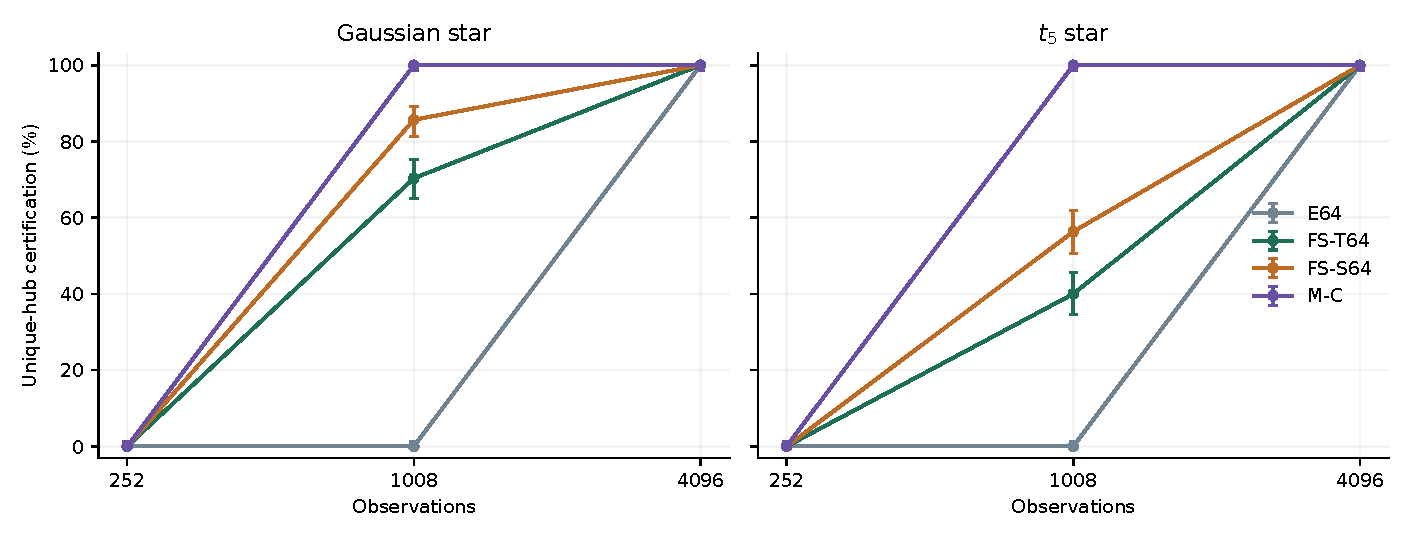
\includegraphics[width=.94\textwidth]{Fig2.pdf}
\caption{Fresh separated-star validation with 300 datasets per point. Error bars are Wilson 95\% intervals. All methods receive the same samples. FS-T64 and FS-S64 reserve 20\% for selection; E64 and M-C use the full sample. M-C is an asymptotic comparator.}\label{fig:power}
\end{figure}

The retained failures are informative. None of the displayed methods certifies a unique hub in the separated stars at $n=252$ or the near-tie stars at either sample size. At $n=4096$, FS-T64 nevertheless excludes on average 9.15 of 12 near-tie vertices from highest degree, versus 0.065 for E64. At $n=1008$, it determines all 12 chain degrees in every one of 200 datasets, compared with no exact degrees for E64. In the two-hub model it excludes on average 8.325 vertices, versus 0.245 for E64. These are distinct structural decisions, not only reductions in interval width.

\section{Ordinal questionnaire application}\label{sec:rse}
We use the public Rosenberg Self-Esteem Scale response data released by the Open-Source Psychometrics Project \citep{rosenberg1965,rse2014}. The data source contains 47974 records. Requiring all ten answers to be in categories 1--4 removes 1428 records; restricting reported age to 18--100 leaves 35079. Q3, Q5, Q8, Q9 and Q10 are reversed as $5-\text{response}$, following the supplied codebook. The graph contains only the ten items, with no total score, fitted latent score or algebraic combination as a node. The archived internal specification records the dataset, these inclusion and reversal rules, the 20\% training fraction and split seed 61023117. It was committed together with the analysis results, so the public archive does not establish prospective specification. No external preregistration was made. Identical response profiles are retained because a short ordinal questionnaire can legitimately produce them; anonymity prevents identifying repeat participation.

The inferential question is which items have certifiably high or low degree in the signed tau-a tree of this response population. Training uses 7015 randomly selected records; the remaining 28064 provide verification. The questionnaire multiplier comparator uses 1999 draws. The source states that included respondents confirmed suitability for research. The Item Response Warehouse lists its release under CC BY 4.0 \citep{irw2026}; our retrieval uses the original data and codebook, with hashes and a download script, and does not redistribute respondent records. IID respondents are an explicit working model. A self-selected anonymous online sample cannot establish representativeness or independently verify repeated participation. Conclusions concern this association target under that model, not latent trait structure or intervention priority.

The application is exploratory. The archive does not independently establish that FS-T64 was designated primary before inspecting application results. We therefore report all 20 variants without a retrospective primary/secondary ranking (Table~\ref{tab:rse-methods}); FS-T64 is used for the detailed structural illustration. Guarantees apply to each fixed procedure separately, not to selecting the most favourable method after observing its results.

\begin{table}[htbp]\centering\small
\caption{All 20 questionnaire procedures on the reported adult sample. No retrospective primary/secondary ranking is imposed. Counts use the same minor and conservation projection. Each exact method has its own nominal 95\% guarantee under IID sampling; the table is not jointly calibrated across methods. M-C is asymptotic. Shared members allows ties; No unique hub means at least two members are certified.}\label{tab:rse-methods}
\begin{tabular}{lrrrr}\toprule
Method & Fixed degrees & Excluded & Shared members & No unique hub\\\midrule
A64 & 6 & 6 & 1 & No\\
E64 & 6 & 6 & 1 & No\\
FS-A64 & 3 & 6 & 0 & No\\
FS-E64 & 8 & 6 & 3 & Yes\\
FS-P & 2 & 2 & 0 & No\\
FS-S64 & 1 & 1 & 0 & No\\
FS-T64 & 8 & 6 & 3 & Yes\\
H-A64 & 6 & 6 & 1 & No\\
H-E64 & 6 & 6 & 1 & No\\
H-P & 3 & 6 & 1 & No\\
H-S64 & 5 & 6 & 1 & No\\
H-T64 & 6 & 6 & 1 & No\\
IUT-A64 & 0 & 0 & 0 & No\\
IUT-E64 & 0 & 0 & 0 & No\\
IUT-P & 0 & 0 & 0 & No\\
IUT-S64 & 0 & 0 & 0 & No\\
IUT-T64 & 0 & 0 & 0 & No\\
M-C & 6 & 6 & 1 & No\\
P & 0 & 0 & 0 & No\\
S64 & 4 & 6 & 0 & No\\
\bottomrule\end{tabular}\end{table}

\begin{table}[htbp]\centering
\caption{Adult questionnaire analysis. Degree and rank bounds are sharp relative to each method\textquotesingle s order relation. FS-T64 uses 7015 training and 28064 verification observations. Its three guaranteed hub members are Q1, Q3 and Q10; Q6 may also attain degree three. No compatible tree has a unique hub.}\label{tab:rse}
\begin{tabular}{lrrrrl}\toprule Item & Sample degree & E64 degree & FS-T64 degree & FS-T64 rank & Guaranteed hub\\\midrule
Q1 & 3 & [3, 3] & [3, 3] & [1, 4] & Yes\\
Q2 & 1 & [1, 1] & [1, 1] & [5, 10] & \\
Q3 & 3 & [2, 3] & [3, 3] & [1, 4] & Yes\\
Q4 & 1 & [1, 1] & [1, 1] & [5, 10] & \\
Q5 & 1 & [1, 1] & [1, 1] & [5, 10] & \\
Q6 & 2 & [2, 3] & [2, 3] & [1, 5] & \\
Q7 & 2 & [1, 2] & [1, 2] & [4, 10] & \\
Q8 & 1 & [1, 1] & [1, 1] & [5, 10] & \\
Q9 & 1 & [1, 1] & [1, 1] & [5, 10] & \\
Q10 & 3 & [3, 4] & [3, 3] & [1, 4] & Yes\\
\bottomrule\end{tabular}\end{table}


FS-T64 retains 111 of the 112 training-ordered path comparisons before stopping. It fixes eight degrees, compared with six under E64, A64 and M-C. In particular, Q3 changes from degree $[2,3]$ to 3 and Q10 from $[3,4]$ to 3. All four methods exclude six items from maximum degree; the gain is a different conclusion about the remaining candidates. E64, A64 and M-C each permit three trees, including one with Q10 as a unique degree-four hub. FS-T64 permits only two, in which Q1, Q3 and Q10 share the maximum degree three. Q6 can join them. Therefore FS-T64 certifies three unavoidable hub members and rules out a unique hub. FS-E64 gives the same degree endpoints here, showing that independently selected testing, rather than the trained stake alone, supplies the application gain.

Enumeration checks every allowed edge subset after lossless screening. An independent Boolean-closure implementation recovers exactly the same accepted trees. A further audit uses the exact spanning-tree polytope and verifies all 110 degree and ordered-pair objectives per method with rational arithmetic. For the four audited adult methods---E64, FS-T64, A64 and M-C---these LP degree and rank endpoints already equal the enumerated endpoints. The displayed conclusions also hold at the minor stage. Thus this example supports targeted statistical calibration and explicit structural reporting, rather than an argument for universally necessary LP complexity.

The all-complete-ages sensitivity analysis has 46546 records. FS-T64 retains four compatible trees, fixes six degrees and still excludes a unique hub; Q1 and Q3 are guaranteed maximum-degree members. Q10 is not guaranteed to share their maximum in this population. This sensitivity concerns a changed response population, not simply additional IID observations from the adult target.

Item tie probabilities in the adult sample range from 0.259 to 0.399. Tau-a measures observed concordance without normalizing away this concentration. As a descriptive sensitivity check, the sample tau-b tree shares eight of nine edges with the tau-a tree: it reallocates one link between Q6 and Q7. The tau-a confidence guarantee is not transferred to tau-b. Marginal association trees also differ from the partial-correlation networks commonly used in psychometrics \citep{epskamp2018}.

The reported analysis uses seed 61023117. As a post-application descriptive check, we generated 100 additional independent training splits, regenerating the associated matching randomization. No favourable split was selected and no conclusions were pooled. Under the common minor and conservation projection, FS-T64 certified Q1, Q3 and Q10 as shared hub members in 16 of 100 runs (Wilson 95\% interval [0.10,0.24]) and excluded a unique hub in the same 16 runs. This interval quantifies Monte Carlo uncertainty over random splits and matchings conditional on the observed dataset. The median number of fixed degrees was six, equal to the original E64 count (interquartile range four to six; range one to eight). In 61\% of runs, every degree and rank interval was contained in its original full-sample E64 counterpart and every E64 guaranteed hub member was retained. Failure of this joint criterion means that a degree or rank interval, or a guaranteed hub member, is not retained. Direct comparison of the archived endpoints confirms that all 39 failing runs lose both a degree bound and a rank bound; 32 also lose guaranteed hub member Q10. Thus the displayed split is favourable, and the three-member conclusion is strongly split-sensitive. Exact enumeration on all 100 retained families agrees with the shared-hub and unique-hub-exclusion decisions. Online Resource 1, Section S10, reports every run and all split variants. The finite-sample guarantee applies to each procedure with its own independently generated split; it does not provide simultaneous coverage across the 100 reruns or across methods.

H-E64 provides a useful counterpoint: it retains all original E64 degree/rank bounds and guaranteed hub members in 94 of the same 100 splits, compared with 61 for FS-T64, but certifies Q1, Q3 and Q10 jointly in only six splits, compared with 16. Thus H-E64 is more stable at preserving the baseline conclusions, while FS-T64 more often reaches the stronger three-member conclusion. This comparison changes both the testing rule and the betting calibration. Holding E64 calibration fixed, H-E64 versus FS-E64 gives retention counts 94 versus 49 and three-member counts six versus ten (Online Resource 1, Table S17). These descriptive comparisons support a trade-off, not uniform superiority of the featured procedure.

The stopping diagnostic identifies the principal bottleneck. In 36 runs the first failed comparison is $\tau_{Q3,Q7}>\tau_{Q6,Q10}$, and in another 36 it is $\tau_{Q3,Q6}>\tau_{Q6,Q10}$. In 37 runs, later comparisons have marginal $p$-values at most 0.05, but the fixed-sequence rule cannot use them after its first failure. Training also changes the reference tree and sequence length (107--127 comparisons). These local ordering failures therefore block potentially informative later steps. Section S10 lists all stopping contrasts and summarizes their positions; the diagnostic reruns reproduce all 100 archived FS-T64 results.

\section{Verification and computational scope}\label{sec:verification}
Independent implementations check the adaptive betting recursion, tied kernels, null expectations over all $3^7$ ternary sequences, agreement of E64 with the existing implementation on continuous data, and complete path certificates on graphs with three through nine vertices. Validation aggregation checks every cell size, seed and dataset-method key. The questionnaire audit verifies all accepted trees twice and checks 880 strong-polytope objectives across eight analyses: E64, FS-T64, A64 and M-C, each applied to the adult sample and to the sample of all complete responses. Exhaustive tests of graphic minors, rank projection and rational bounds are retained in the supplement.

The selected family contains $\sum_{e\notin T_0}|P_{T_0}(e)|$ comparisons, at most $(m-p+1)(p-1)$ on a complete graph. Training tau-a estimates require $O(p^2n_0\log n_0)$ work using tie-safe sweeps. Direct evaluation of the selected matching evidence costs $O(RN K_T)$, where $K_T$ is its directed family size. Exact subset-polytope descriptions and tree enumeration are used only for small graphs or strongly screened families. The supplementary timing audit remains descriptive; subsecond differences are not the principal evidence of practical benefit. No large-$p$ scalability claim is inferred from the ten-item application.

For the questionnaire, median wall times over five warmed sequential runs on an AMD EPYC 9V74 80-Core Processor were 0.038 s for training/selection, 1.902 s for shared 64-matching evidence, 4.0 ms for order construction, 1.8 ms for the FS-T64 minor projection, 0.572 s for its 110 strong-polytope LP objectives with rational checks, and 0.6 ms for exact enumeration. Training/selection, evidence evaluation and order construction serve all 15 split variants; minor projection, the strong-LP audit and exact enumeration concern FS-T64 only. Data loading and compilation are excluded; environment details and every timing are in Section S10 and the archive. The minor projection and exact enumeration audit together take about 2.4 ms (0.13\% of the shared evidence-evaluation time); the optional LP adds 0.57 s without changing the degree, rank or hub conclusions in this application.

\section{Discussion}
The main improvement is a measurable increase in useful finite-sample decisions after independent selection. It changes separated-star hub certification at 1008 observations and establishes shared hubs in the reported split of a real ordinal dataset. The latter conclusion recurs in 16\% of additional splits, so the application demonstrates a possible gain rather than a stable improvement across randomizations. The questionnaire result also illustrates why a unique-hub success indicator alone can be misleading: the data can certify that several vertices share the maximum, making non-uniqueness the supported conclusion.

The questionnaire trade-off is explicit: H-E64 more reliably preserves the E64 conclusions, whereas FS-T64 more often certifies three shared members. The intended decision therefore matters when choosing a procedure before verification.

Selection has a cost. It discards training observations from verification, and an early weak or false comparison can stop the sequence before other useful ones. Fixed fractions can be mismatched to small gaps, and the selected scheme has no universal power advantage. At short samples and near-tied leaders, unique-hub inference remains difficult. Full-U-statistic multiplier inference is more powerful in the evaluated separated stars, with asymptotic rather than finite-sample calibration. Variance-sensitive inequalities for full U-statistics \citep{peel2010} remain a substantive alternative; this study does not claim to have implemented or surpassed them.

A possible route to greater split stability is to average valid e-values for each common, prespecified hypothesis across splits, following the derandomisation principle illustrated by \citet{ren2024}; the changing selected families and sequences here require an explicit FWER-valid aggregation rule, which remains future work.

Optimization and statistics address separate losses. The Abalone enumeration improves several endpoints that even a stronger connectivity LP leaves unchanged. In the questionnaire, the selected relation is already informative enough for minor-stage decisions. Rational certificates verify the numerical inequalities, while exact compatible-tree sets explain which structural ambiguity remains. The scientific interpretation still depends on the chosen correlation target and sampling model.

\section*{Statements and Declarations}
\subsection*{Funding}No dedicated funding was received for this study.
\subsection*{Competing interests}The authors declare no relevant competing interests.
\subsection*{Compliance with Ethical Standards}
This study is a secondary analysis of publicly released, anonymous questionnaire responses. No participants were recruited or contacted and no identifying information was collected by the authors. The original source states that only respondents who confirmed that their responses were accurate and could be used for research were included.
\subsection*{Consent for publication}
No individual identifying information is reported.
\subsection*{Data availability}Simulation designs, per-dataset results, questionnaire retrieval instructions, original-source hashes, derived summaries and verification scripts accompany the article. Raw questionnaire responses and third-party price histories are not redistributed. The supplementary UCI applications retain their original attribution.
\subsection*{Supplementary information}
Online Resource 1: supplementary comparisons and sensitivity analyses, including additional calibrations, morphometric examples, computational timings and Polish-market diagnostics.
\subsection*{Code availability}\ifanonymous Reproducibility materials and immutable identifiers are supplied separately.\else Reproducibility code, comparison relations and complete replication results are archived at the immutable revision \url{https://github.com/mgalazka84/gpw-hub-reliability/tree/22ddc926c06abe271b62cfa81af96cfb0159564f/contrast_inference/power_revision}.\fi
\subsection*{Declaration of generative AI and AI-assisted technologies in the manuscript preparation process}The authors used ChatGPT/Codex (OpenAI) to assist with writing code. The authors reviewed and tested the code and take full responsibility for the content of the article.
\subsection*{Author contributions}
\ifanonymous The authors jointly contributed to the research and manuscript preparation and take responsibility for its scientific content.\else Marek Gałązka and Hanna Wdowicka jointly contributed to the research and preparation of the manuscript. Both authors take responsibility for its scientific content.\fi
\setlength{\bibsep}{0pt}
\bibliographystyle{plainnat}
\begingroup\small\bibliography{references,new_references}\endgroup
\end{document}
